\section{Auswertung}
\subsection{Fourier-Amplituden}
Die Fourier-Amplituden wurden alle bei einer Frequenz von $50\, kHz$ gemessen
 für die Rechteckspannung werden die Amplituden mit der Formel
\begin{equation}
  a_k = \frac{A \cdot 4}{k \pi}
\end{equation}
bestimmt.Dabei werden nur ungerade $k \in \mathds{N}$ betrachtet.
Für alle ungeraden $k$ gilt, $a_k =0$. \\
$A$ ist eine Konstante.
$a_k - c_k$  sind fortlaufend gewählte Bezeichnungen für die Koeffizienten.

\begin{table}[h]
\centering
\caption{Rechteckspannung}
\label{tab:reck}
\begin{tabular}{c c c c c}
\toprule
$a_k$ & $U_{gemessen}/V$ & $U_{berechnet(A=1,64)}/V$ & $Differenz/ \% $\\
\midrule
$a_1$ & 2,090 & 2,088 & 0,096 \\
$a_3$ & 0,720 & 0,696 & 3,333 \\
$a_5$ & 0,400 & 0,418 & 4,500 \\
$a_7$ & 0,312 & 0,298 & 4,487 \\
$a_9$ & 0,200 & 0,232 & 16,00 \\
\bottomrule
\end{tabular}
\end{table}
\newpage
Für die Sägezahnspannung ergeben sich die Amplituden mit der Formel:
\begin{equation}
  b_k = \frac{2}{k} \, .
\end{equation}
Hier werden gerade und ungerade $k \in \mathds{N}$ betrachtet.
\begin{table}[h]
\centering
\caption{Sägezahnspannung}
\label{tab:säge}
\begin{tabular}{c c c c}
\toprule
$b_k$ & $U_{gemessen}[V]$ & $U_{berechnet}[V]$ & $Differenz[ \% ]$ \\
\midrule
$b_1$ & 2,100 & 2,000 & 4,762\\
$b_2$ & 0,968 & 1,000 & 3,306\\
$b_3$ & 0,736 & 0,667 & 9,375\\
$b_4$ & 0,552 & 0,500 & 9,420\\
$b_5$ & 0,392 & 0,400 & 2,041\\
$b_6$ & 0,336 & 0,300 & 10,714\\
$b_7$ & 0,312 & 0,286 & 8,333\\
$b_8$ & 0,264 & 0,250 & 5,303\\
$b_9$ & 0,208 & 0,200 & 3,846\\
\bottomrule
\end{tabular}
\end{table}
Die Amplituden der Dreieckspannung ergeben sich durch
\begin{equation}
  c_k = \frac{C\cdot 4}{\pi k^2} \, .
\end{equation}
Es werden wieder nur ungerade $k$ $\in$ $\mathds{N} $ betrachtet.
$C$ ist eine frei wählbare Variable.
\begin{table}[h]
\centering
\caption{Dreieckspannung}
\label{tab:drei}
\begin{tabular}{c c c c c}
\toprule
$c_k$ & $U_{gemessen}[V]$ & $U_{berechnet(C=2,1)}[V]$ & $Differenz[\% ]$ &
$U_{berechnet(C=1)}[V]$\\
\midrule
$c_1$ & 2,660 & 2,674 & 0,526 & 1,273\\
$c_3$ & 0,312 & 0,297 & 4,808 & 0,141\\
$c_5$ & 0,096 & 0,107 & 11,458 & 0,051\\
$c_7$ & 0,052 & 0,055 & 5,769 & 0,026\\
$c_9$ & 0,026 & 0,033 & 26,923 & 0,016\\
\bottomrule
\end{tabular}
\end{table}
\newpage
\subsection{Fourier Synthese}
In den folgenden Abbidungen (\ref{fig:reck}), (\ref{fig:säg}) und (\ref{fig:drei})
sind die synthetisierten Funktionen der Rechteck- ,Sägezahn- und Dreiecksschwinung zu sehen.
Die Anfangsspannung beträgt $613\, V$. \\
Mit
\begin{equation}
  a_k = \frac{613}{k} \,\, ,k \in \mathds{N}
  \label{eqn:for}
\end{equation}
werden die Spannungen für die einzelnen Einstellungen bestimmt.
Dies geschieht mit den selben $k$,
wie bei der Amplitudenbestimmung.
\begin{figure}[h]
\centering
\begin{subfigure}{0.48\textwidth}
\centering
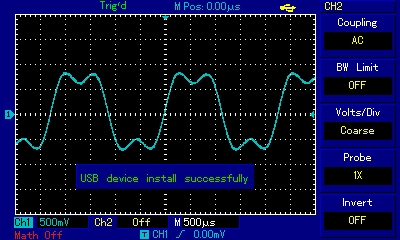
\includegraphics[height=3.75cm]{MAP003.jpg}
\label{fig:reck1}
\end{subfigure}
\begin{subfigure}{0.48\textwidth}
\centering
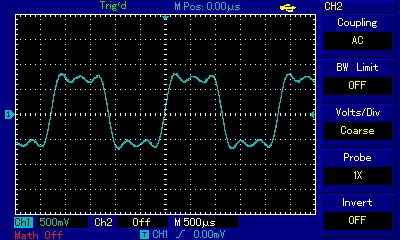
\includegraphics[height=3.75cm]{MAP004.jpg}
\label{fig:reck2}
\end{subfigure}
\begin{subfigure}{0.48\textwidth}
\centering
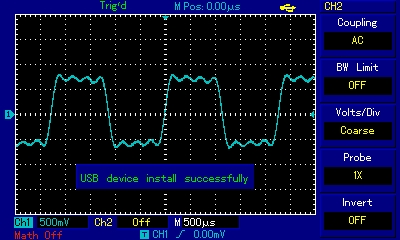
\includegraphics[height=3.75cm]{MAP005.jpg}
\label{fig:reck3}
\end{subfigure}
\begin{subfigure}{0.48\textwidth}
\centering
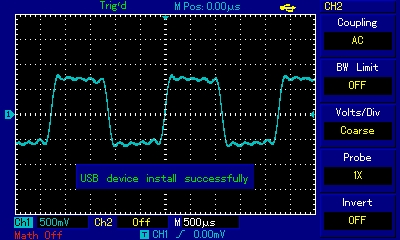
\includegraphics[height=3.75cm]{MAP006.jpg}
\label{fig:reck4}
\end{subfigure}
\caption{Rechteckspannung}
\label{fig:reck}
\end{figure}
\\
Für die Spannungen der Sägzahnschwingung, wird ebenfalls Formel (\ref{eqn:for}) verwendet.
\begin{figure}[h]
\centering
\begin{subfigure}{0.48\textwidth}
\centering
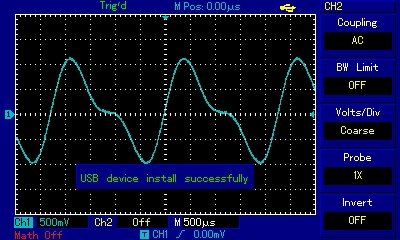
\includegraphics[height=3.75cm]{MAP007.jpg}
\label{fig:säg1}
\end{subfigure}
\begin{subfigure}{0.48\textwidth}
\centering
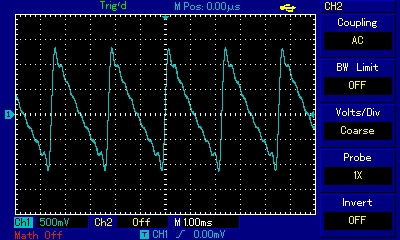
\includegraphics[height=3.75cm]{MAP010.jpg}
\label{fig:säg4}
\end{subfigure}
\begin{subfigure}{0.48\textwidth}
\centering
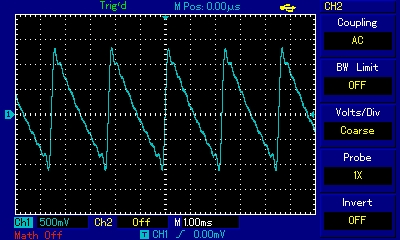
\includegraphics[height=3.75cm]{MAP011.jpg}
\label{fig:säg5}
\end{subfigure}
\caption{Sägezahnspannung}
\label{fig:säg}
\end{figure}

Es sind zum Teil Unebenheiten in der Rechteck- und Sägezahnspannung zu sehen.
Dies lässt sich mit dem Gibbschen Phänomen erklären.\\
\FloatBarrier
Für die Dreieckspannung wird die Formel
\begin{equation}
  c_n = \frac{613}{k^2} \, \, , k \in \mathds{N}
\end{equation}
verwendet.
\begin{figure}[h]
\centering
\begin{subfigure}{0.48\textwidth}
\centering
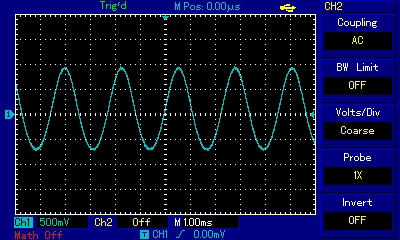
\includegraphics[height=3.75cm]{MAP012.jpg}
\label{fig:drei1}
\end{subfigure}
\begin{subfigure}{0.48\textwidth}
\centering
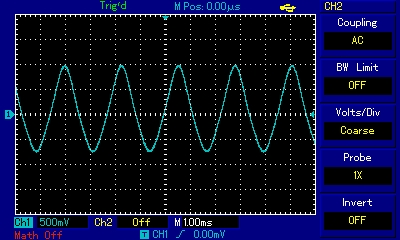
\includegraphics[height=3.75cm]{MAP014.jpg}
\label{fig:drei2}
\end{subfigure}
\caption{Dreieckspannung}
\label{fig:drei}
\end{figure}

\section{Disskusion}
Die Messung der Ampituden ist durch den Messvorgang am Oszillosgraphen fehlerbehaftet.
Bei dem zweiten Teil der Messungen
konnten für die Dreieckssannung nur Bilder für die ersten beiden Spannungen gemacht werden,
da die Spannungen sehr schnell sehr klein wurden und es nicht möglich war diese einzustellen.
Zusammenfassend kann gesagt werden, dass die Messungen die Theorie sehr gut wiederspiegelt.
